\section{Exp1: Simulated experiment}

A task in a simulated environment was learned first to see whether a NAF neural
network could learn to move the end-effector (eef) to arbitrarily set goal positions.
\subsection{Environment}

A simulated environment was set up to allow for changing the position of an eef
by giving 2-d relative movement commands. The area that was considered allowed
to work within was a $0.15 \times 0.30$ m area and commands sending the eef
outside this area gave a reward of $-2$. For all other successor states the
rewards were set to $\exp\left(-1000|\mathbf{x}_e - \mathbf{x}_g|^2\right) - 1$
where $\mathbf{x}_e$ is the eef pose and $\mathbf{x}_g$ is the goal pose. This
makes the reward equal $0$ close to the goal and rapidly decay to $-1$ further
from the goal. Commands with norm larger than $5$ cm were capped. No noise were
added to movements and the environment was reset when reaching the outside of
the area or getting within a $1$ cm radius of the goal. When resetting the
environment, eef and goal poses were randomly sampled within the defined area.
The goal pose remains the same until the environment is reset. After commanding
some action on the environment, the successor state was returned. This included
the new eef pose and the goal pose.

\subsection{Algorithms}

The same layout of the network was used as described in section
\ref{sec:distributed_naf} with two hidden layers of $100$ outputs each. The
$\mathbf{\mu}$ output had a $\tanh$ function scaled by $0.1$ as activation. All
poses were 2-dimensional where eef and goal pose were concatenated as input to
the network. A discount factor was set to $0.98$ and the Adam optimizer
\cite{kingma2014adam} was used with learning rate $0.0001$ on a batch size of
$512$. The replay buffer was sampled from as described in section
\ref{sec:prio_sampling} with $\alpha = 1$ and $\beta$ in iteration $i$ out of a
total amount of iterations $i_{tot}$ was set according to:

\begin{equation}
    \beta_i = \exp \left( 10(i - i_{tot}) / i_{tot}\right)
\end{equation}

For sampling, a binary tree was used where the value of a parent equals the sum
of its children \cite{schaul2015prioritized}. This way, drawing one sample
from a total of $N$ samples is $\mathcal{O}(\log_2(N))$. The exact procedure is
to first draw a sample from $U(0, \sum_i p_i)$ and then start from the top of
the tree and recurse down to the corresponding leaf node. The loss was defined
as the mean square error of the temporal-difference errors.

\subsection{Results}

\begin{figure}[h]
    \centering
    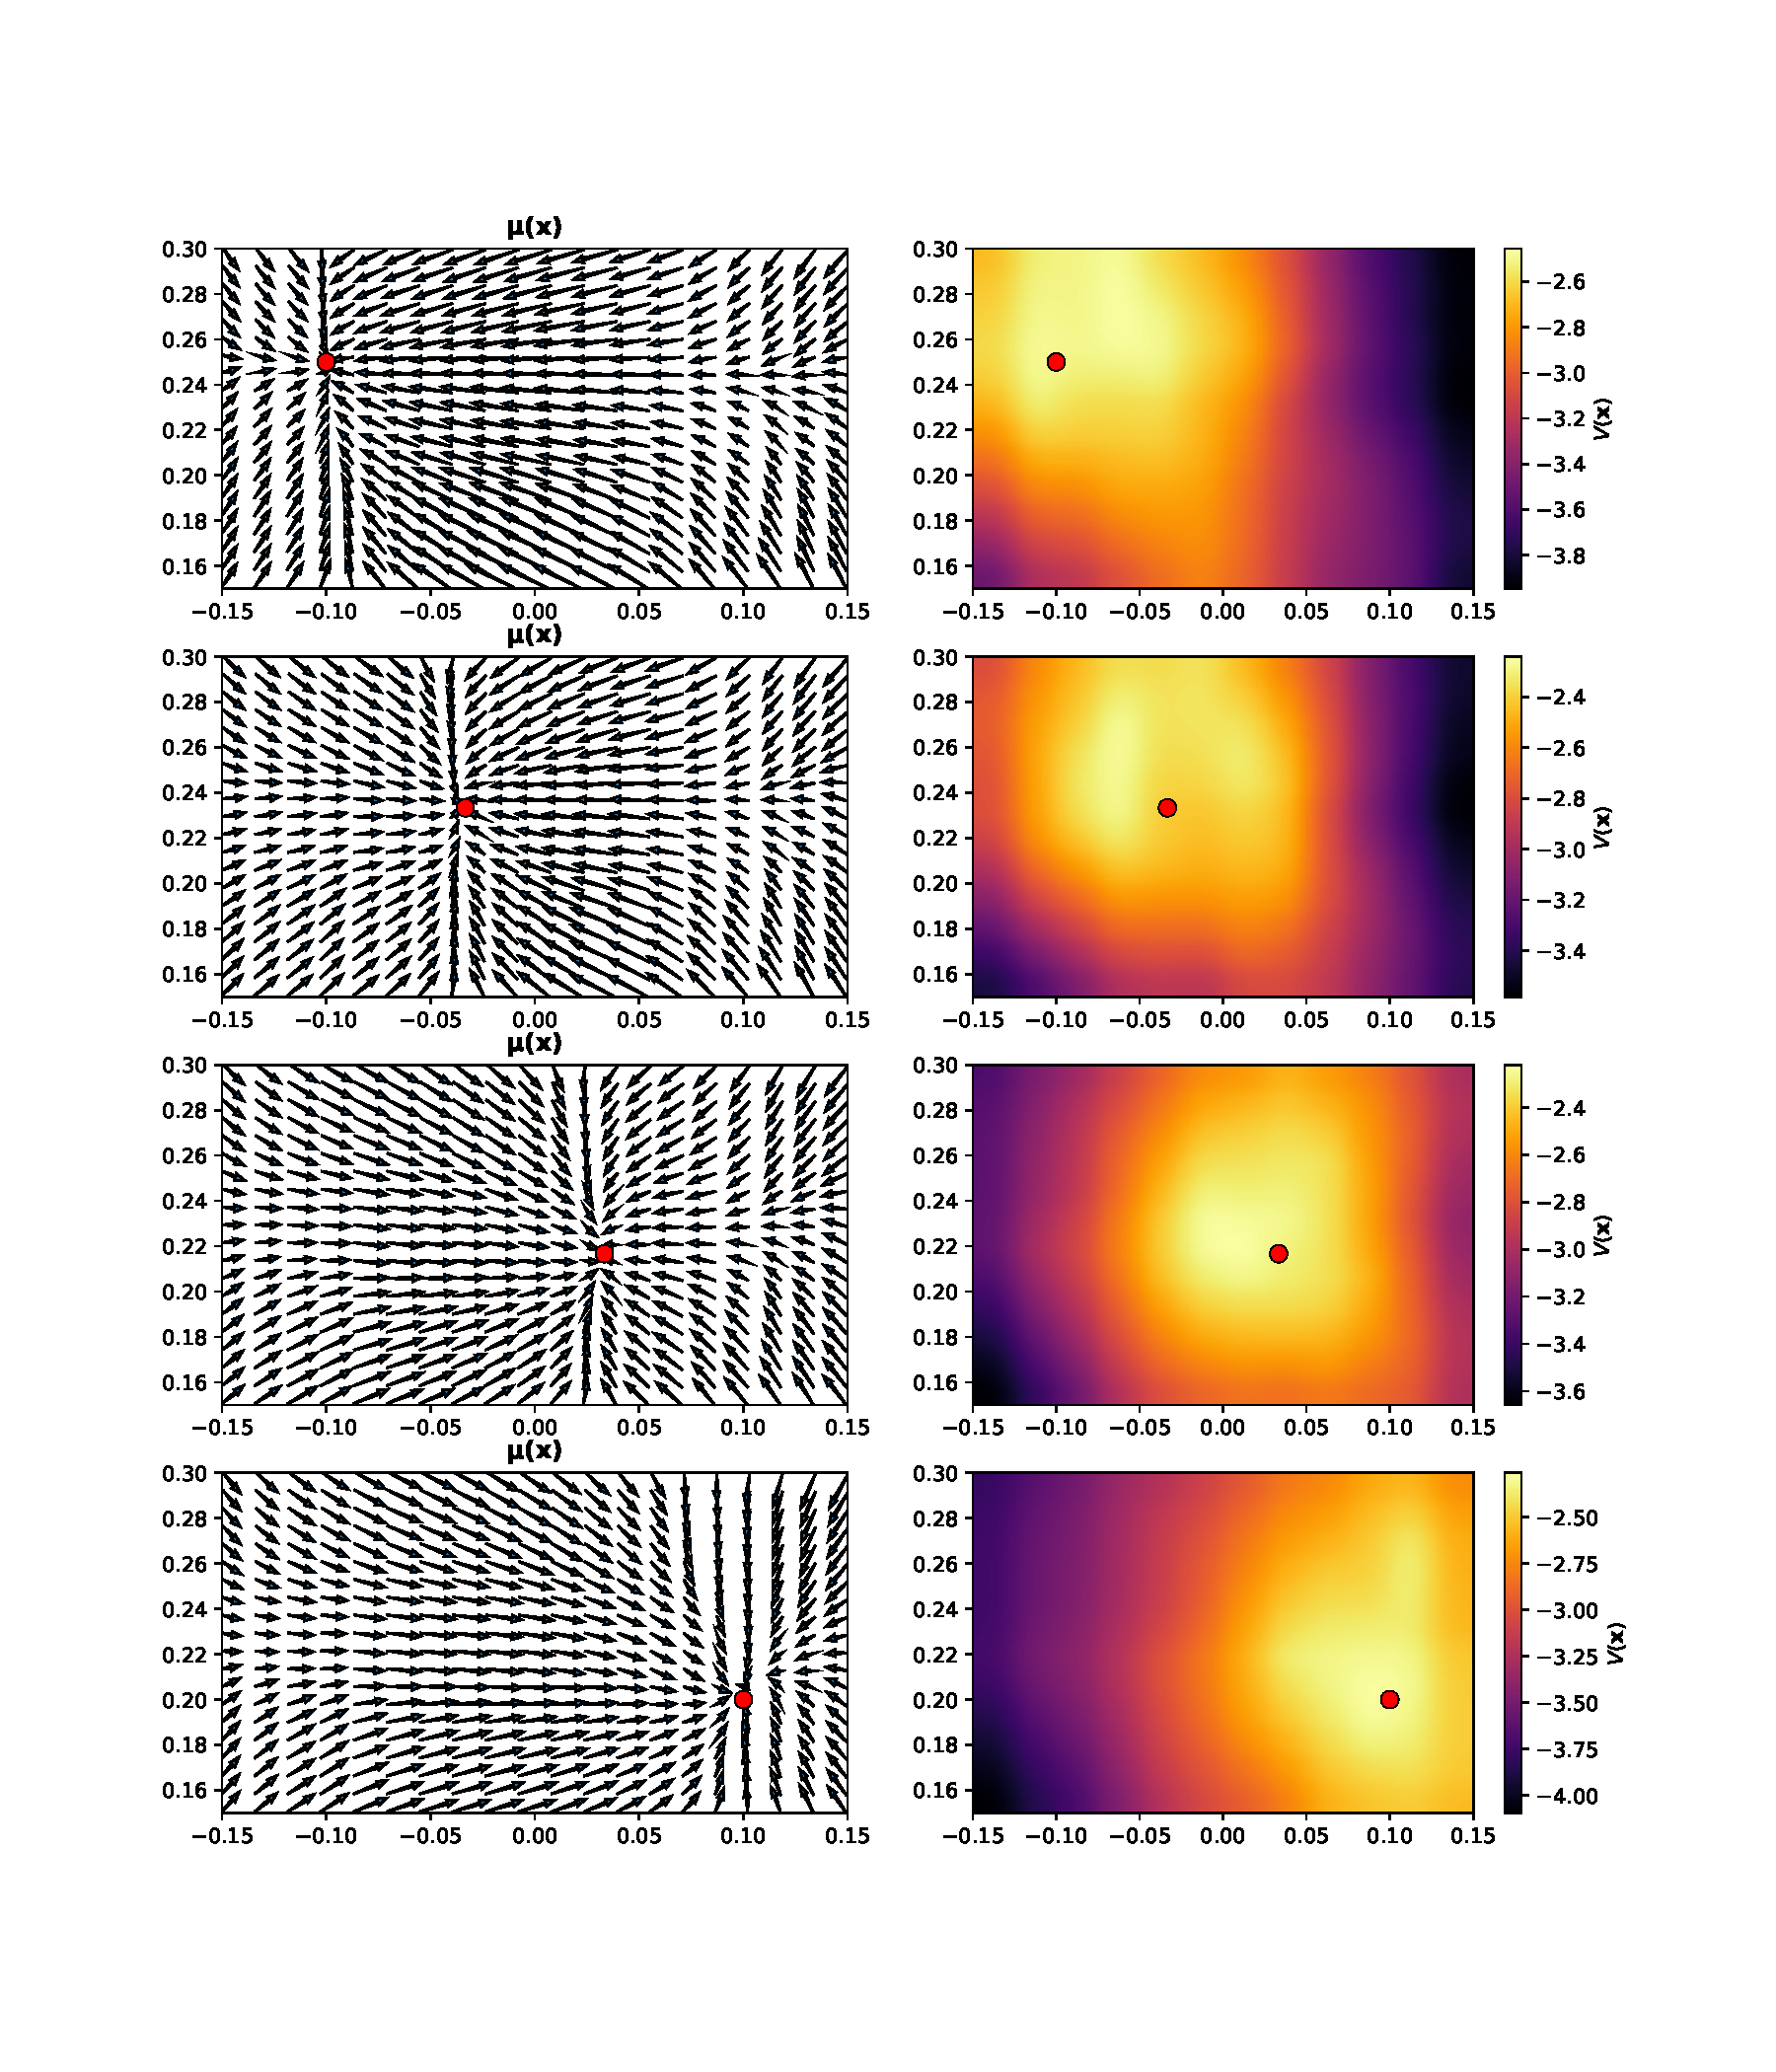
\includegraphics[width=\textwidth]{res/moving_goal_summary.pdf}

    \caption{Trained policy and value function for moving an end-effector to
    randomly set goals. Vertical and horizontal axes are end-effector
    positions. Red dot is goal position. Left figure shows the learned policy
    $\mu$, right side shows the learned value function for different goal
    poses.}
    
\end{figure}

\begin{figure}[h]
    \centering
    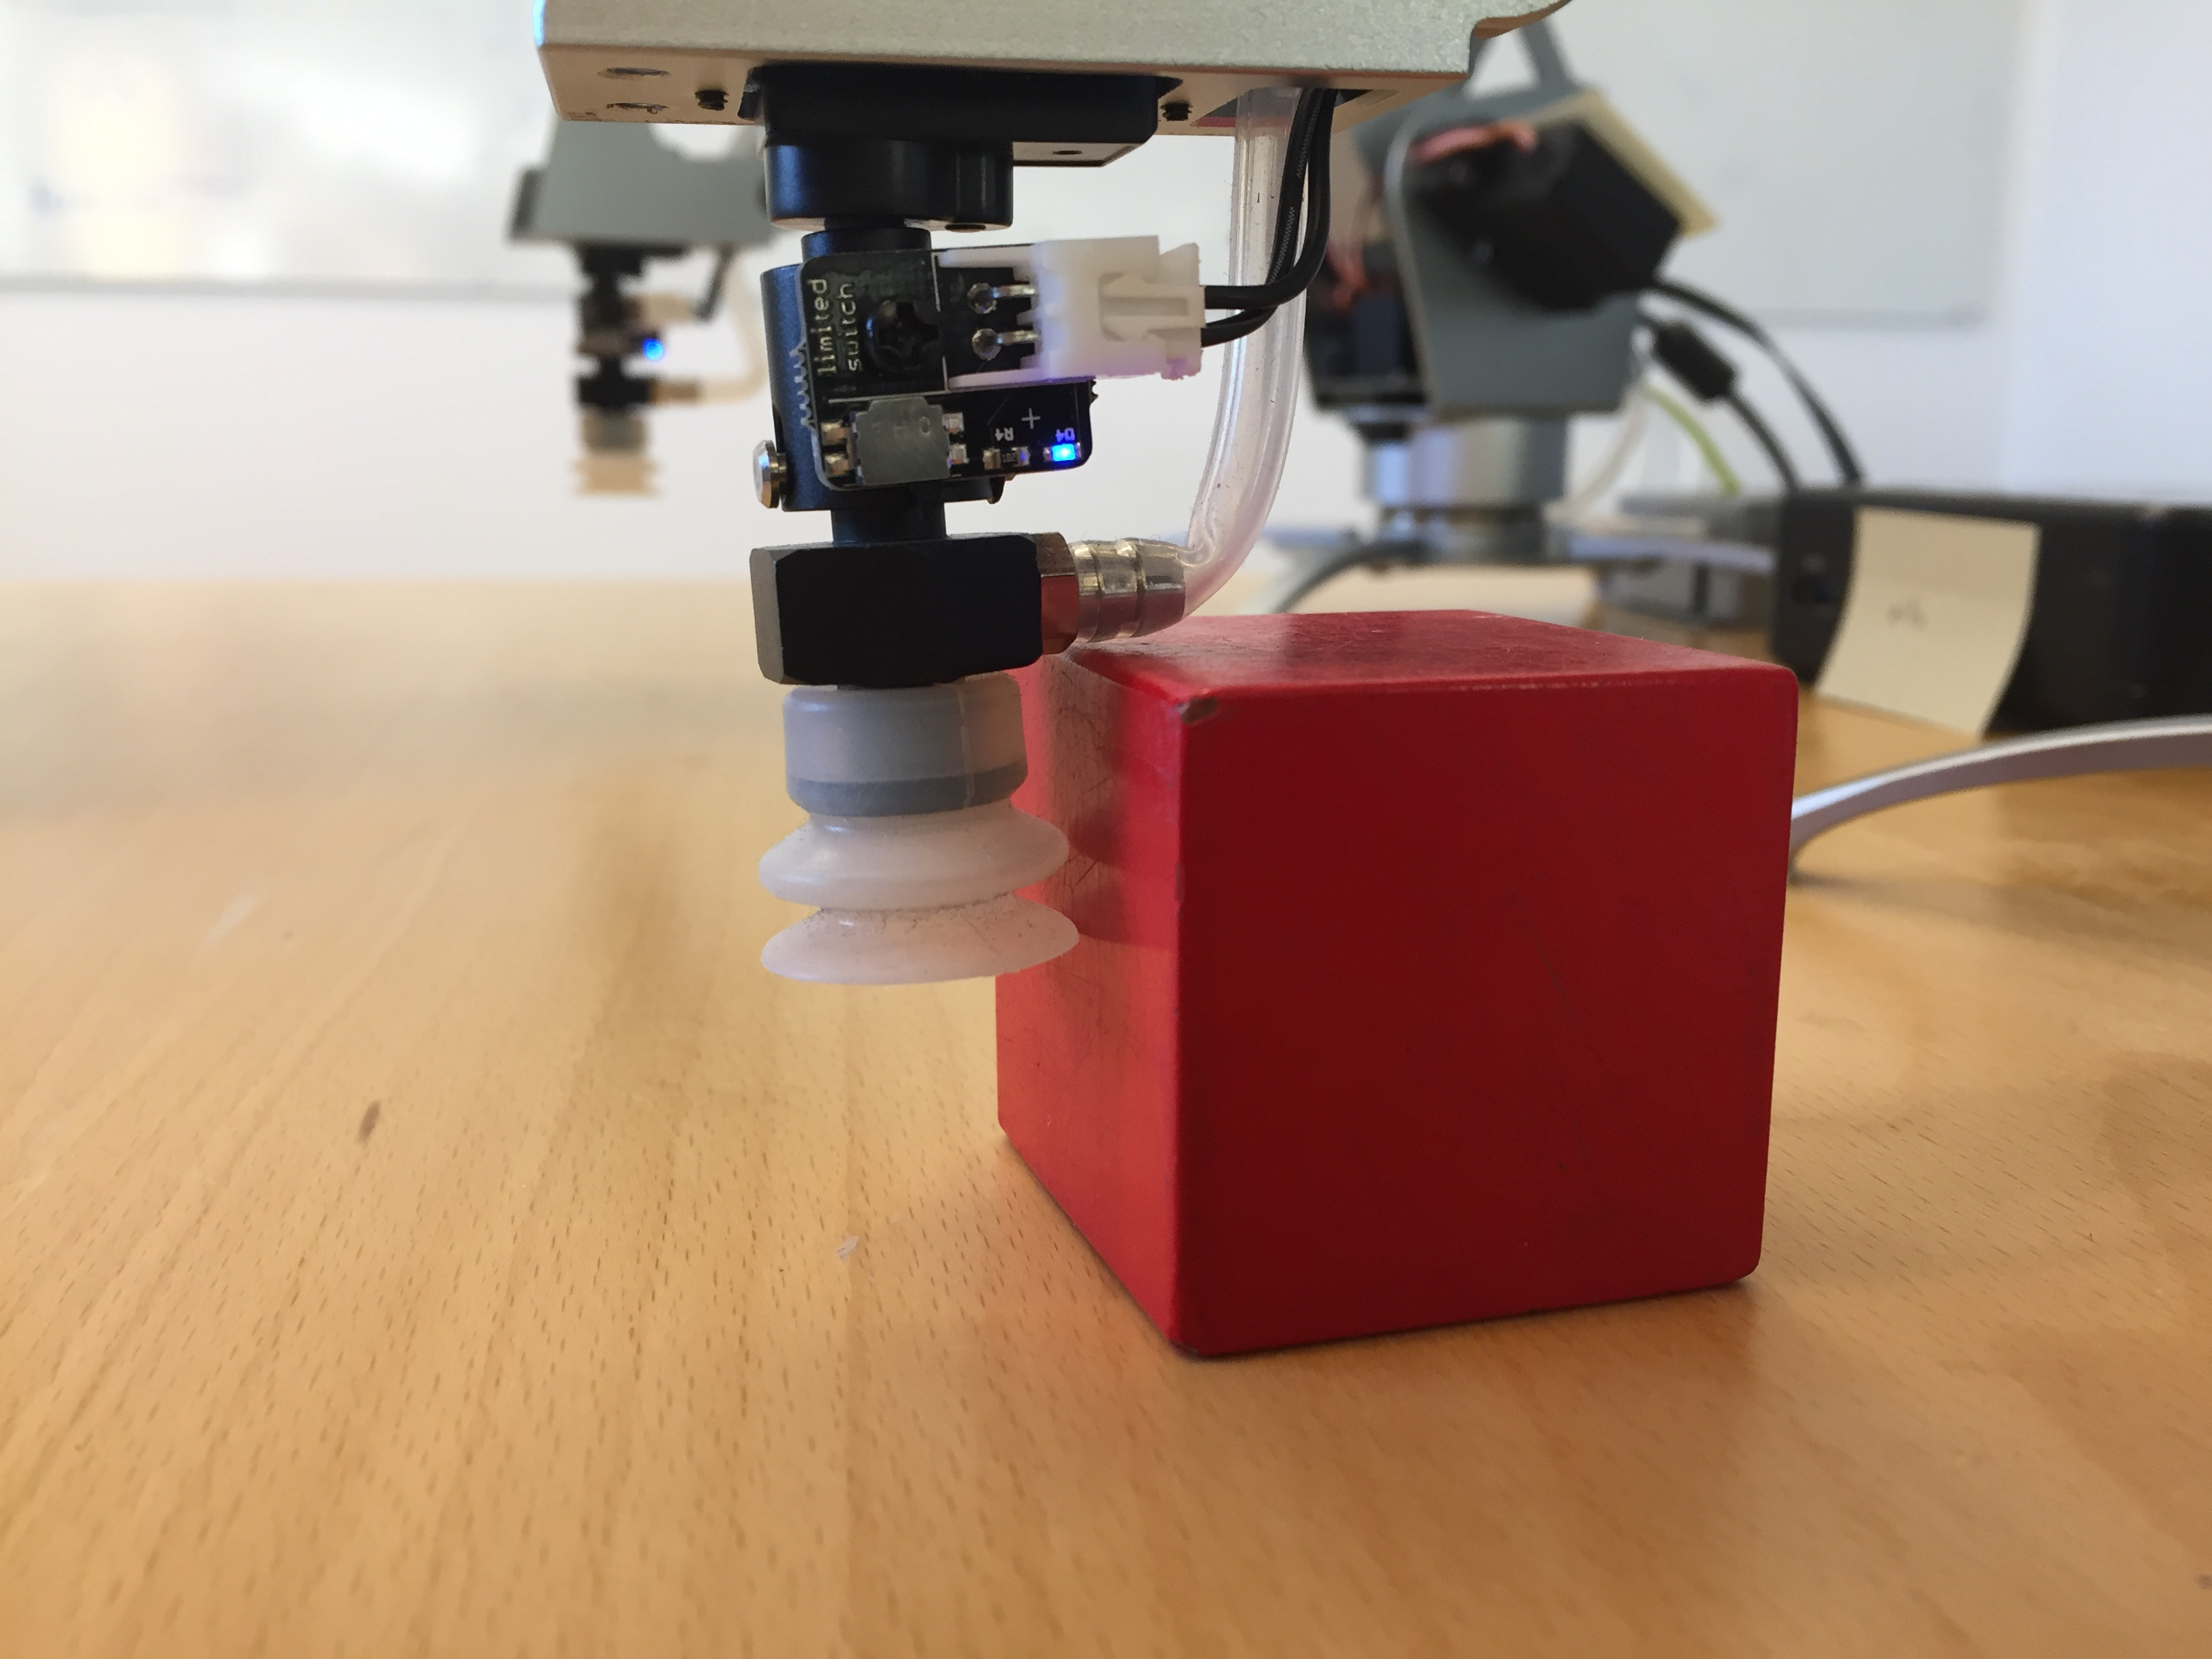
\includegraphics[width=0.40 \textwidth]{res/eef_cube_low.jpg}
    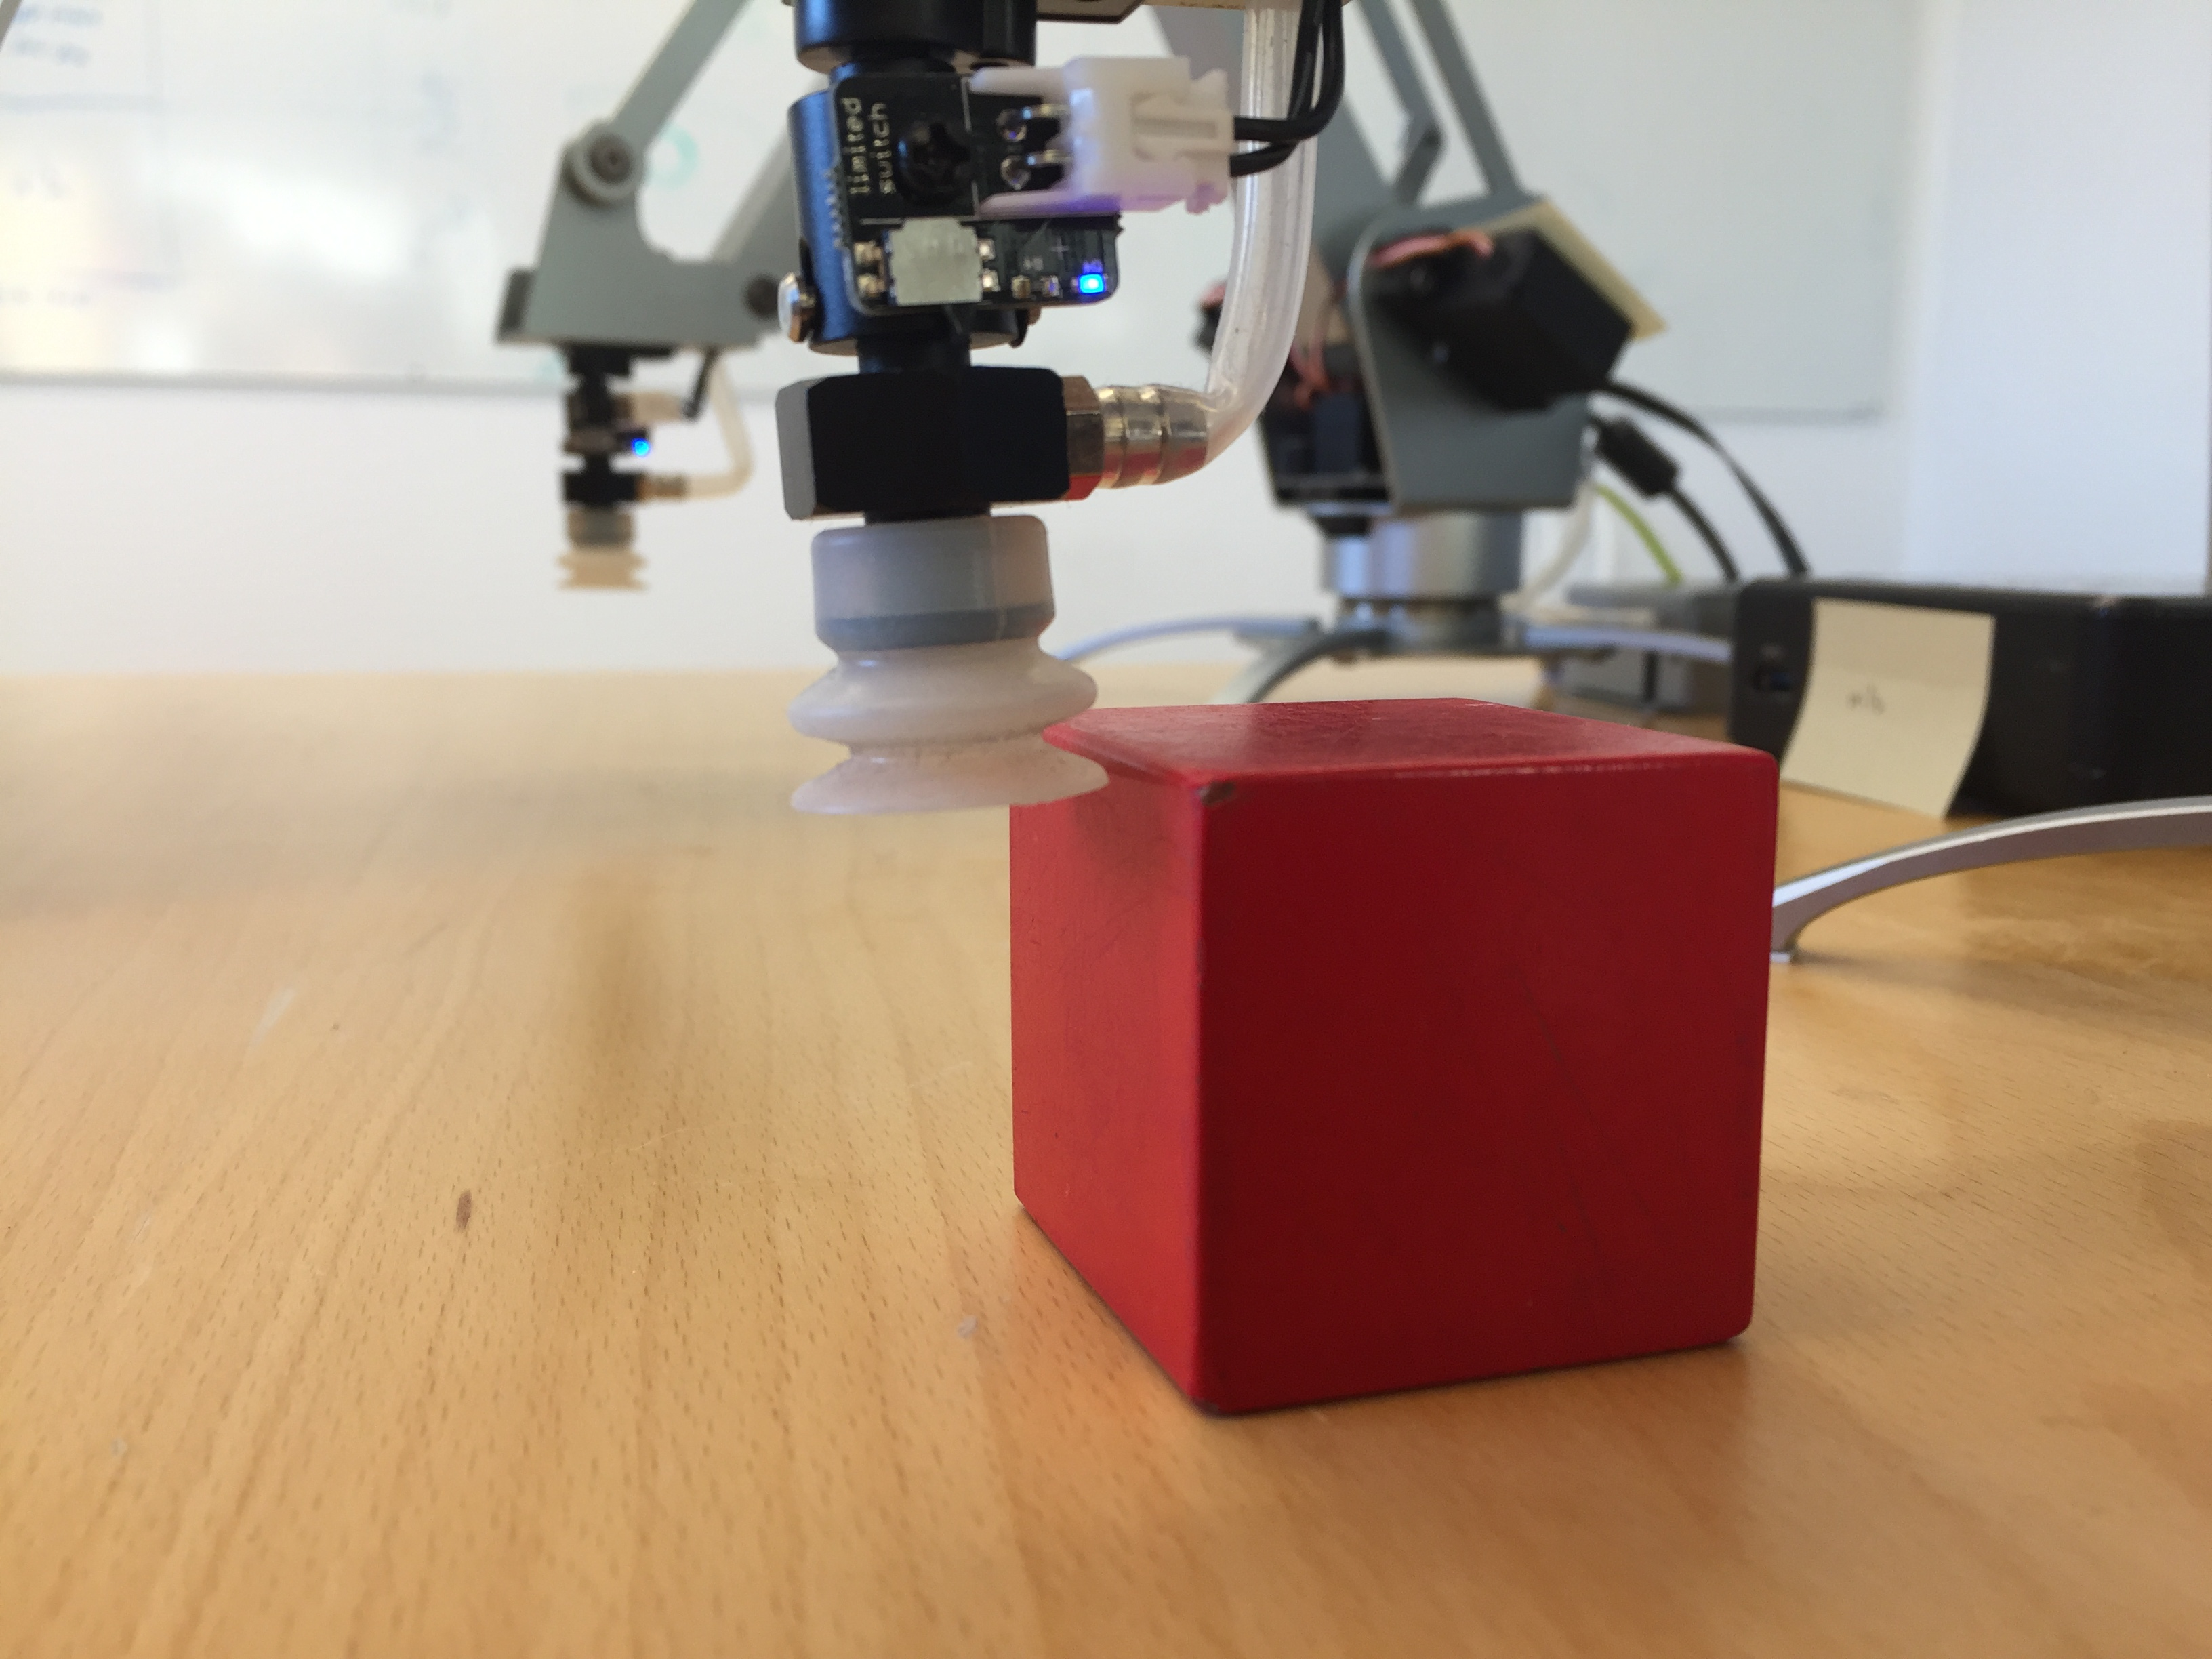
\includegraphics[width=0.40 \textwidth]{res/eef_cube_high.jpg}

    \caption{Possible $z$-values of the eef. TODO: Finish/polish this}
    
\end{figure}
